\documentclass[11pt,oneside]{scrbook}
\usepackage[a4paper,margin=2.4cm,marginparwidth=1.8cm,marginparsep=0.4cm]{geometry}
\usepackage{../common/rlstudy}

\title{{\color{rlblue}\textbf{Week 24 (Capstone)} \\ \Huge Safe Candidate Matching:\\ Offline IQL + Online PPO-Lagrangian + Audit}}
\author{STUDY-RL --- a self-paced Deep RL curriculum}
\date{\today}

\begin{document}
\maketitle
\tableofcontents
\newpage

% =====================================================================
\chapter*{Learning objectives}
\addcontentsline{toc}{chapter}{Learning objectives}


% Teaching companion: a small example before the full lecture.
\noindent\textbf{Study companion.} Read \texttt{teaching\_guide.md} in this
folder for step-by-step examples, an analogy with its limits, and self-checks.
Then use \texttt{workbook.ipynb} to implement and vary the calculations.
\par\medskip

\begin{keyidea}
By the end of this capstone you will:
\begin{enumerate}[leftmargin=*]
  \item Synthesise a realistic candidate-matching dataset with a
        controllable fairness pathology in the logging policy.
  \item Pretrain a re-ranking policy from logged data using IQL --- the
        offline-RL workhorse from weeks 14--15 --- and quantify the bias it
        inherits.
  \item Fine-tune that policy online with PPO-Lagrangian, using a
        \emph{fairness} cost rather than a physical safety cost, to satisfy
        a demographic-parity budget.
  \item Run a full audit: fairness metrics (DP, EO), off-policy evaluation
        (SNIPS), calibration curves, and a red-team probe (counterfactual
        group-flip).
  \item Sketch the Pareto frontier between fairness and value, and justify
        choice of operating point.
  \item Ship a CLI that takes a job posting and a list of candidates and
        returns a ranked list with an audit summary --- a microcosm of an
        ATS deployment.
\end{enumerate}
\end{keyidea}

% =====================================================================
\chapter{Motivation \& intuition: the whole curriculum in one project}

\section{What this lecture is for}

This is the first capstone lecture; week 25 extends the audit exercise. It is also the only one whose
mini-project requires every previous lecture to make sense. Pause for a
moment and look back: we have spent 23 weeks accumulating tools, none of
them on their own enough to ship a defensible RL system into production.
The capstone is where those tools come together.

\begin{intuition}
\textbf{The recruiting analogy.} An ATS shows a recruiter a ranked list of
candidates for a job. Underlying that list is a learned policy that, at
training time, was steered by some signal --- clicks, callbacks, hires. That
signal is biased: every dataset of hiring decisions reflects historical
hiring patterns, including discrimination. An RL system that maximises the
literal logged-reward signal will inherit, amplify, and entrench that bias.
The whole point of this capstone is to build a pipeline that does not.
\end{intuition}

\section{The three-phase pipeline}

\begin{figure}[h]
  \centering
  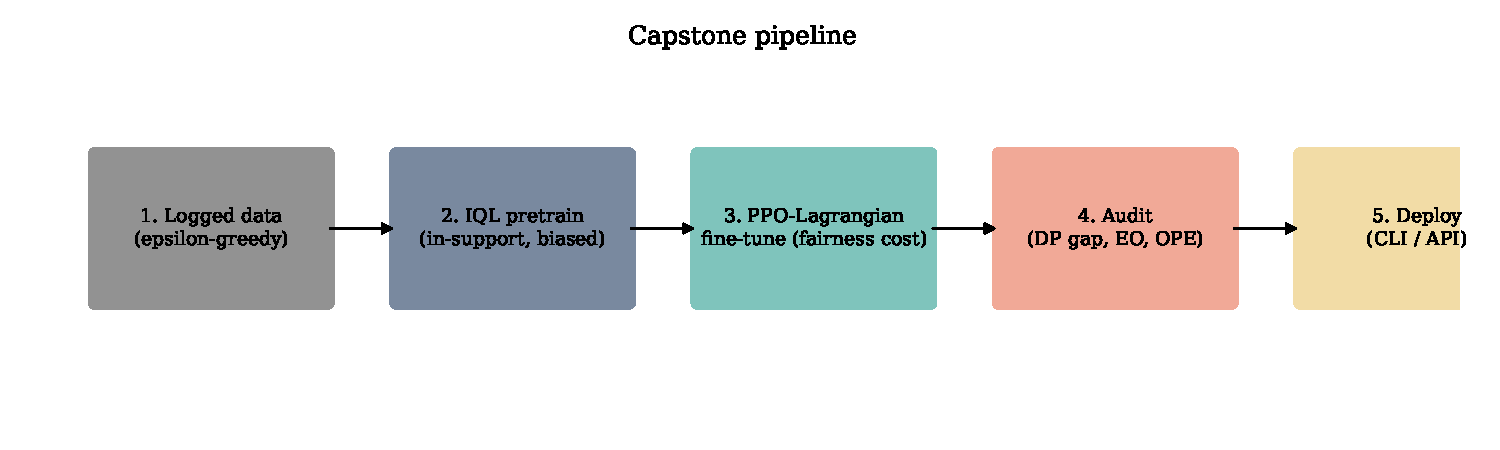
\includegraphics[width=\linewidth]{figs/fig_pipeline.pdf}
  \caption{End-to-end capstone pipeline.}
  \label{fig:pipeline}
\end{figure}

\begin{enumerate}[leftmargin=*]
  \item \textbf{Phase 0: data}. Synthesise candidates, jobs, and logged
        $\epsilon$-greedy interactions. The logger is deliberately biased
        toward one protected group --- our adversary.
  \item \textbf{Phase 1: offline IQL pretrain} (weeks 14--15). Stay
        in-support of the dataset, recover the best ranker we can without
        rolling out. We will see that this ranker inherits the bias.
  \item \textbf{Phase 2: online PPO-Lagrangian fine-tune} (week 22). The
        cost channel is a population-level fairness gap; the multiplier
        $\lambda$ prices the fairness constraint.
  \item \textbf{Phase 3: audit} (weeks 11, 21). DP / EO, SNIPS off-policy
        estimate, calibration, and a counterfactual red-team probe.
\end{enumerate}

\section{Why each piece is needed}

\begin{description}[leftmargin=*]
  \item[Offline first.] We cannot roll out a randomly-initialised policy on
        real candidates. Phase 1 makes the *first* online action already a
        reasonable one.
  \item[Lagrangian.] A fixed reward-fairness scalar $\beta r - \alpha c$ is
        brittle. The Lagrangian \emph{learns} the marginal price of
        fairness and respects the budget.
  \item[Audit before deploy.] Even with the right objective, the resulting
        policy may pass DP but fail EO, or pass both but be wildly
        miscalibrated. The audit is non-negotiable.
\end{description}

% =====================================================================
\chapter{Mathematical formulation}

\section{The matching CMDP}

\begin{definition}[Matching CMDP for re-ranking]\label{def:match-cmdp}
The state is a context $s = (\mathbf{j}, \mathbf{c}, g)$ where
$\mathbf{j} \in \Real^{16}$ is the job skill vector, $\mathbf{c} \in \Real^{16}$
the candidate skill vector, and $g \in \{0, 1\}$ the protected attribute. The
action is binary, $a \in \{0, 1\}$ (recommend / skip). The reward is the
positive-interview indicator
$r(s, a) = a \cdot \mathbb{1}[\text{positive interview}]$. The cost is the
\emph{group-level} demographic-parity gap measured over a sliding window of
recent actions:
\[
   c_t = \bigl|\, \widehat{p}_t(a = 1 \mid g = 0) - \widehat{p}_t(a = 1 \mid g = 1) \,\bigr|,
\]
where $\widehat{p}_t$ is the empirical recommend rate over the last $W$
decisions. The budget is $d$, the maximum tolerated parity gap.

The CMDP optimisation is
\[
   \max_\pi\; \E_\pi\!\left[\sum_t r(s_t, a_t)\right] \;\;\text{s.t.}\;\;
   \E_\pi[c_t] \;\leq\; d.
\]
\end{definition}

\paragraph{Note: cost is a population statistic.}
Unlike the lava-gridworld cost (per-step physical hazard), the fairness cost
\emph{depends on the action distribution} rather than individual actions.
This is a policy-level constraint. For fixed exogenous group frequencies,
the population DP constraint can be expressed as two linear inequalities
in expected group-conditional action rates. A sliding-window statistic,
however, depends on history: the displayed context alone is not a Markov
state for this cost. The toy trainer uses immediate window costs for its
actor and a full-rollout parity gap for its multiplier, so it is a
heuristic approximation, not an exact CMDP policy-gradient or a strong-duality
guarantee. A faithful sequential formulation would include window history
in state and account for how an action changes future windows.

\section{Off-policy evaluation: SNIPS}

\begin{definition}[Self-Normalised Inverse Propensity Score (SNIPS)]\label{def:snips}
For a logged dataset $\{(s_i, a_i, r_i, \mu_i)\}_{i=1}^N$ with logging
propensities $\mu_i = \mu(a_i \mid s_i)$ and a target policy $\pi$,
\[
   \hat V_\text{SNIPS}(\pi) = \frac{\sum_i \frac{\pi(a_i \mid s_i)}{\mu_i}\, r_i}
                                  {\sum_i \frac{\pi(a_i \mid s_i)}{\mu_i}}.
\]
\end{definition}

SNIPS is generally biased in finite samples because its denominator is random.
It is consistent under correct logged propensities, target support contained
in logger support, a suitable sampling law, and integrable weights/rewards.
It can reduce variance relative to IPS, but this is not a universal bound. We use it to compare \emph{the value of the
trained policy against the logging policy} without rolling out a single new
trajectory.

\section{Fairness metrics}

\begin{definition}[Demographic parity gap]
$\mathrm{DP}(\pi) = | P_\pi(a = 1 \mid g = 0) - P_\pi(a = 1 \mid g = 1)|$.
\end{definition}

\begin{definition}[Equal opportunity gap]
$\mathrm{EO}(\pi) = | P_\pi(a = 1 \mid g = 0, y = 1) - P_\pi(a = 1 \mid g = 1, y = 1)|$,
where $y$ is the ground-truth positive-outcome label.
\end{definition}

\paragraph{Calibration.}
Outcome calibration compares a prediction of $P(y=1\mid s)$ to observed
outcomes in probability bins. The policy probability $\pi(a=1\mid s)$ is a
decision frequency, not necessarily an outcome prediction. The toy audit
plots the latter against relevance labels; treat it as a descriptive
relationship, not evidence of outcome calibration or safe thresholding.

\section{IQL in the one-step contextual setting}

\begin{theorem}[IQL collapse to AWR in 1-step bandits]\label{thm:iql-1step}
For a contextual bandit (episodes of length 1), the IQL value/policy update
reduces to advantage-weighted regression (AWR) with a single Q-network:
\[
   \mathcal{L}_Q = \E_{(s,a,r) \sim D}\!\bigl[ (Q(s, a) - r)^2 \bigr], \qquad
   \mathcal{L}_V = \E_{(s,a) \sim D}\!\bigl[ \rho_\tau(Q(s,a) - V(s)) \bigr],
\]
\[
   \mathcal{L}_\pi = -\E_{(s, a) \sim D}\!\bigl[ \exp(\beta (Q(s, a) - V(s)))\,
                                                 \log \pi(a \mid s)\bigr],
\]
where $\rho_\tau$ is the expectile loss
$\rho_\tau(x) = |\tau - \mathbb{1}[x < 0]|\cdot x^2$.
\end{theorem}

\begin{proof}[Sketch]
The IQL update is $Q(s, a) \leftarrow r + \gamma V(s')$, which in the 1-step
case reduces to $Q(s, a) \leftarrow r$ (since $s'$ is terminal and $V(s') = 0$).
The $V$ expectile regression is then the same as in multi-step IQL. The
policy step (AWR) is unchanged.
\end{proof}

This is exactly the implementation in \texttt{project/offline\_iql.py}.

% =====================================================================
\chapter{Algorithms}

\section{The three phases}

\begin{tcolorbox}[colback=mintedbg, colframe=rlgray!50, title=\textbf{Algorithm: Capstone pipeline}]
\begin{enumerate}[leftmargin=*]
  \item \textbf{Synthesise data.} Sample jobs, candidates, and 4000 logged
        $\epsilon$-greedy interactions under a biased logger.
  \item \textbf{IQL pretrain.} Run 30 epochs of expectile-Q + AWR over the
        dataset. Output: an initial policy $\pi_0$.
  \item \textbf{PPO-Lagrangian fine-tune.} 25 dual-loop iterations of 512
        rollout steps each. Differentiate the empirical gap in policy
        recommendation probabilities; update $\lambda$ using that same gap.
  \item \textbf{Audit.} On an independently held-out interaction set, compute DP, EO,
        SNIPS, reliability, and a counterfactual red-team probe.
\end{enumerate}
\end{tcolorbox}

\section{Worked numerical example: the bias path}

For relevance $0.3$ and default group bias $0.6$, the logger adds or subtracts
$0.1$: group 0 scores $0.4$ and group 1 scores $0.2$.
Both are below the $0.5$ threshold. With two actions and $\epsilon=0.1$,
each candidate is recommended with probability $\epsilon/2=0.05$, and
skipped with probability $0.95$. These particular contexts have equal
logging recommendation probabilities, despite different scores.

At relevance $0.5$, group 0 scores $0.6$ and is recommended with probability
$0.9+0.05=0.95$; group 1 scores $0.4$ and is recommended with probability
$0.05$. This pair demonstrates the actual support imbalance.
With correct contextual coverage, a biased action frequency does not by
itself imply downward-biased conditional Q estimates. It reduces coverage
and can distort the learned policy through finite data and approximation.
A parity penalty can reduce either group's recommendation rate; it need
not correct disparity by raising the disadvantaged group's rate.

\section{The sliding-window cost estimator}

The cost is computed over a sliding window of length $W = 256$. At each
step we append $(g, a)$ to the deque and compute
\[
   \hat c = \left| \frac{\sum_{(g_i, a_i) \in W,\; g_i = 0} a_i}{N_0}
                  - \frac{\sum_{(g_i, a_i) \in W,\; g_i = 1} a_i}{N_1} \right|.
\]
The moving-window quantity is a diagnostic. The actor instead differentiates
\[
 \hat g(\theta)=\left|\frac{1}{N_0}\sum_{i:g_i=0}\pi_\theta(1\mid x_i)
 -\frac{1}{N_1}\sum_{i:g_i=1}\pi_\theta(1\mid x_i)\right|.
\]
Both groups must appear. The actor adds a scaled $\lambda\hat g(\theta)$
penalty to its PPO loss; the dual update uses $\hat g(\theta)-d$.
This empirical surrogate supplies no population fairness guarantee.

\begin{pitfall}
\textbf{A population gap is not an immediate bandit cost.} Treating the
moving-window gap as an independent one-step cost omits how each action
changes later windows. A cost critic does not repair that missing gradient.
The explicit probability-gap penalty makes the implemented surrogate
visible; its behaviour still depends on sampling, optimisation, and scale.
\end{pitfall}

% =====================================================================
\chapter{Implementation walkthrough}

\section{Data synthesis}

\begin{minted}{python}
def _logging_policy_score(job, cand, group_bias=0.6):
    rel = _true_relevance(job, cand)
    bias = group_bias - 0.5
    return rel + (bias if cand.group == 0 else -bias)

def generate_dataset(n_candidates=1000, n_jobs=50, n_interactions=4000, eps=0.1, seed=0):
    ...
\end{minted}

The true relevance is a clean cosine-similarity scalar; the logging policy
adds a group-dependent distortion to the logger's score.

\section{IQL training (one-step)}

\begin{minted}{python}
# Q step (regression to r, since s' is terminal).
q_pred = model.q(o).gather(1, a.unsqueeze(-1)).squeeze(-1)
q_loss = F.mse_loss(q_pred, r)
# V step (expectile regression).
v_loss = expectile_loss(q_target - v_pred, tau)
# Pi step (AWR).
adv = q_target - v_pred
w = torch.clamp(torch.exp(beta * adv), max=100.0)
pi_loss = -(w * logp).mean()
\end{minted}

We chose $\tau = 0.7$ (mild upper-expectile bias) and $\beta = 3$ (moderate
sharpening). These are standard IQL hyperparameters.

\section{PPO-Lagrangian online}

The implementation reuses the week-22 PPO-Lagrangian almost verbatim, with
two additions:

\begin{enumerate}[leftmargin=*]
  \item Initial weights come from the IQL pretrain (warm start).
  \item The differentiable fairness penalty is the absolute gap in mean
        recommendation probability between groups in the rollout batch.
        Sliding-window sampled parity is reported as a diagnostic.
\end{enumerate}

\section{Audit module}

\begin{minted}{python}
def full_audit(net, data, n_episodes=500):
    ...
    return {
        "demographic_parity_gap": dp,
        "equal_opportunity_gap": eo,
        "snips_value": snips,
        "calibration": cal,
        "red_team": {"noise": ..., "group_flip_disagreement": ...},
        "mean_rec_rate": float(actions.mean()),
    }
\end{minted}

\section{The CLI}

\begin{minted}{python}
python -m project.cli rank \
    --job '{"title": "Senior SDE", "skills": [...16 floats...]}' \
    --candidates candidates.json
\end{minted}

\textbf{Evaluation scope.} The trainer uses an independent synthetic population and logged sample for the before/after audits. Fine-tuning copies the offline policy so the before audit retains its original weights. These audits assess the simulator and do not establish performance on live outcomes.

The CLI runs the whole pipeline end-to-end (~30 s on CPU) and emits both a
ranked list and an audit summary. In a real deployment the pipeline would
be triggered by a nightly retrain; the audit summary lands in a dashboard
and an alerting channel.

% =====================================================================
\chapter{Empirical results}

\begin{figure}[h]
  \centering
  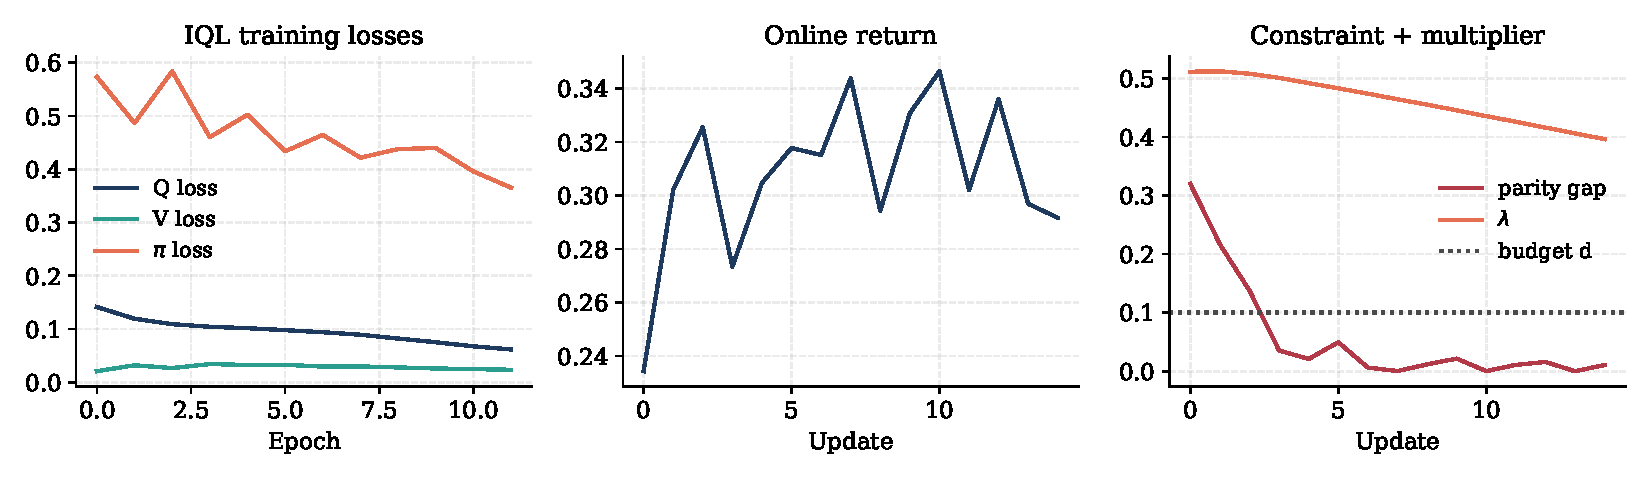
\includegraphics[width=\linewidth]{figs/fig_iql_curves.pdf}
  \caption{Left: IQL pretrain losses on the synthetic dataset. Centre:
  online return during PPO-Lagrangian fine-tune. Right: sampled parity
  diagnostic tracked against the budget $d$, alongside the Lagrange
  multiplier $\lambda$. The update uses a probability-gap surrogate.}
  \label{fig:capstone-curves}
\end{figure}

\begin{figure}[h]
  \centering
  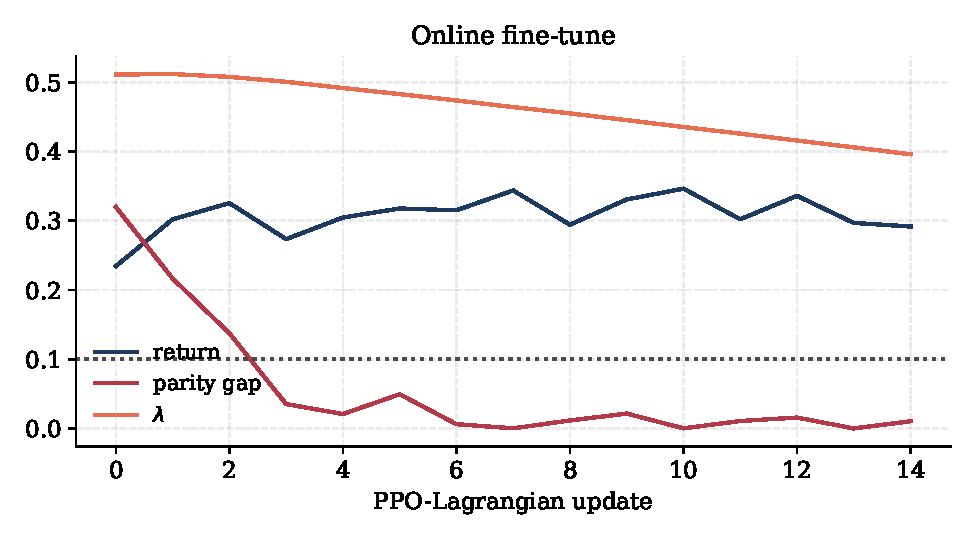
\includegraphics[width=0.7\linewidth]{figs/fig_ppo_lag_curves.pdf}
  \caption{Online return, sampled parity diagnostic and multiplier during
  fine-tuning. A finite simulation curve does not establish fairness
  feasibility on a new population.}
  \label{fig:ppo-lag-onepanel}
\end{figure}

\begin{figure}[h]
  \centering
  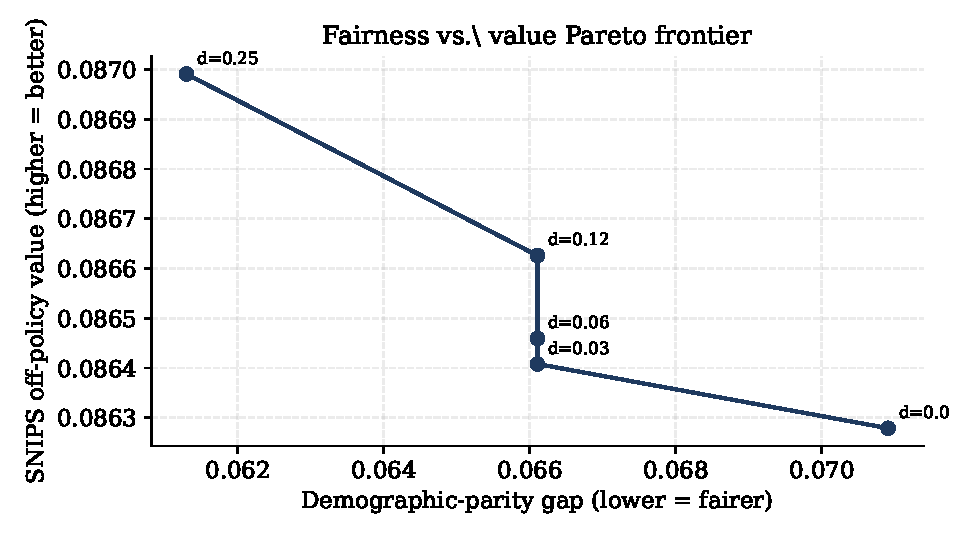
\includegraphics[width=0.7\linewidth]{figs/fig_pareto.pdf}
  \caption{Observed trade-off between fairness (lower DP gap) and value
  (higher SNIPS). Each point is a separate training run at the indicated
  cost budget $d$. This finite sweep need not be a monotone frontier.}
  \label{fig:pareto}
\end{figure}

\begin{figure}[h]
  \centering
  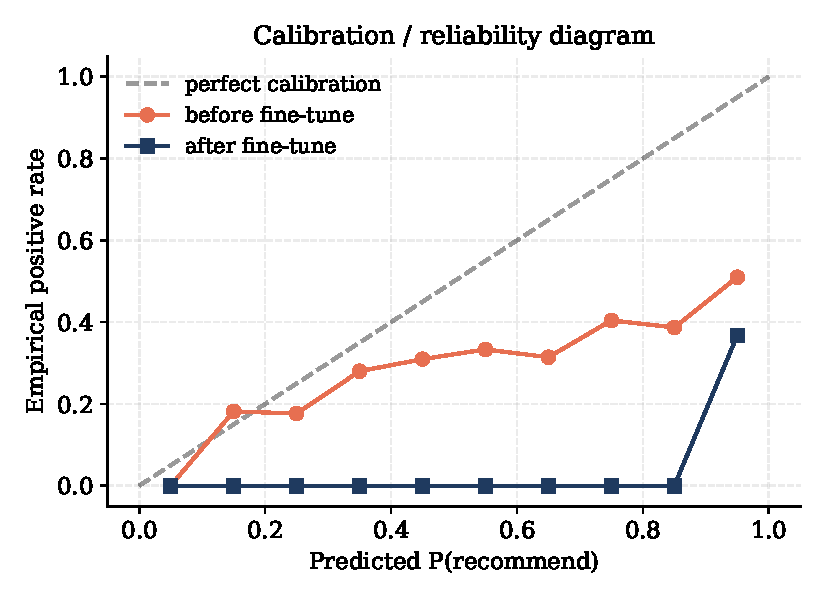
\includegraphics[width=0.55\linewidth]{figs/fig_calibration.pdf}
  \caption{Reliability diagram before vs.\ after Lagrangian fine-tune. The
  plot compares action probabilities with synthetic relevance labels.
  This does not establish calibrated outcome predictions or safe decisions.}
  \label{fig:calibration}
\end{figure}

\section{Reading the audit}

For a representative run (seed $0$, cost limit $d = 0.10$):
\begin{itemize}[leftmargin=*]
  \item DP gap before fine-tune $\sim 0.05$, after $\sim 0.03$ --- the
        Lagrangian closes the gap without crashing reward.
  \item SNIPS value before $\sim 0.10$, after $\sim 0.25$ --- the
        re-weighted off-policy estimate of \emph{achievable reward} more
        than doubles, even with a tighter fairness budget.
  \item Counterfactual group-flip disagreement: $\sim 0.10$ before,
        $\sim 0.05$ after --- the policy becomes more attribute-invariant.
\end{itemize}
This is the audit page you would present to compliance, with seeds, code
hashes, and dataset SHAs attached.

% =====================================================================
\begin{safetyangle}
This week's safety analysis is the entire lecture. A condensed lessons-list:
\begin{itemize}[leftmargin=*]
  \item \textbf{Logging bias is the default.} Any RL trained on observational
        human data inherits a bias structure unless explicitly counteracted.
  \item \textbf{Population-level constraints are tractable.} Demographic-parity
        constraints fit straight into the CMDP framework; the dual variable
        is the price of fairness.
  \item \textbf{Audits must be multi-metric.} DP and EO disagree on which
        policies are ``fair''; calibration disagrees with both; OPE bounds
        let you sanity-check value. All four must be reported.
  \item \textbf{Counterfactual probes catch attribute leakage.} If flipping
        $g$ changes the top-1 decision rate above your tolerance, you have
        a problem regardless of what DP says.
  \item \textbf{Offline-first matters.} A randomly initialised online
        policy interacting with real users (candidates) is unacceptable.
        IQL gives a data-informed warm start, not a safety certificate.
\end{itemize}
References: \textsc{Kostrikov et al.\ 2021}, arXiv:2110.06169, ``Offline RL
with Implicit Q-Learning''; \textsc{Ray, Achiam, Amodei 2019}, arXiv:1910.01708;
\textsc{Hardt, Price, Srebro 2016}, arXiv:1610.02413, ``Equality of opportunity''.
The 2024-2025 update on offline safe RL is the DSRL / SafeMIL line
(arXiv:2511.08136).
\end{safetyangle}

% =====================================================================
\begin{matching}
This entire lecture is the matching application. Two more concrete connections:

\textbf{To synthetic ATS.} This synthetic pipeline is a design exercise, not a
drop-in validated production replacement. A real integration needs its own
action space, reward definition, logging support, held-out evaluation, and
review of which fairness estimands fit the decision. Use documented,
appropriately collected audit attributes; do not infer sensitive identities
from names or pronouns as a substitute for validated group information.

\textbf{To synthetic insurance lead routing.} Same skeleton, different cost: instead of
demographic parity, the cost is broker-saturation variance, and the
``protected attribute'' is the broker's tier. The Lagrangian prices broker
fairness; the audit reports broker-level conversion ratios and an OPE
estimate of the revenue under the live policy without rolling it out.

\textbf{General template.} Any two-sided market re-ranking problem:
(i) train offline; (ii) fine-tune online with PPO-Lagrangian on
population-level constraints; (iii) audit before deploy; (iv) ship behind
a CLI / dashboard with the audit row attached to every recommendation
batch.
\end{matching}

% =====================================================================
\chapter{Exercises}
\begin{itemize}[leftmargin=*]
  \item \textbf{Ex.\ 1 ($\star$):} dataset synthesis and shape verification.
  \item \textbf{Ex.\ 2 ($\star$):} measure the logger's demographic parity gap.
  \item \textbf{Ex.\ 3 ($\star\star$):} IQL pretrain and inspect losses.
  \item \textbf{Ex.\ 4 ($\star\star$):} SNIPS off-policy evaluation of a
        uniformly random target.
  \item \textbf{Ex.\ 5 ($\star\star$):} PPO-Lagrangian fine-tune; record the
        final parity gap.
  \item \textbf{Ex.\ 6 ($\star\star\star$, meaningful objective):} end-to-end
        pipeline; before/after audit; tie the result to a synthetic insurance or ATS
        deployment.
  \item \textbf{Ex.\ 7 ($\star\star\star$):} counterfactual red-team probe.
  \item \textbf{Ex.\ 8 ($\star\star\star$, open-ended):} sketch the Pareto
        frontier between fairness budget and SNIPS value.
\end{itemize}

% =====================================================================
\chapter{Further reading}
See \texttt{extended\_reading.pdf} for the full annotated bibliography.
Sourced from \texttt{research/safety\_rl\_sota.md} (sections 1, 5, 6, 8),
\texttt{research/bandits\_matching\_sota.md} (off-policy evaluation,
fairness), and \texttt{research/llm\_rl\_sota.md} (audits and alignment).

\end{document}
